\chapter{Workloads}
\label{section:workloads}

\section{Query Description Format}
\label{sub:queries_structure}
Queries are described in natural language using a well-defined structure that consists of three sections:
\textit{description}, a concise textual description of the query;
\textit{parameters}, a list of input parameters and their types;
and \textit{results}, a list of expected results and their types.
The syntax used in \textit{parameters} and \textit{results} sections is as follows:

\begin{itemize}
    \item \textbf{Entity}: entity type in the dataset.\\
        One word, possibly constructed by appending multiple words together, starting with uppercase character and following the camel case notation,
        \eg \texttt{TagClass} represents an entity of type ``TagClass''.
    \item \textbf{Relationship}: relationship type in the dataset.\\
        One word, possibly constructed by appending multiple words together, starting with lowercase character and following the camel case notation,
        and surrounded by arrow to communicate direction,
        \eg \texttt{-worksAt->} represents a directed relationship of type ``worksAt''.
    \item \textbf{Attribute}: attribute of an entity or relationship in the dataset.\\
        One word, possibly constructed by appending multiple words together, starting with lowercase character and following the camel case notation,
        and prefixed by a ``.'' to dereference the entity/relationship,
        \eg \texttt{Person.firstName} refers to ``firstName'' attribute on the ``Person'' entity,
        and \texttt{-studyAt->.classYear} refers to ``classYear'' attribute on the ``studyAt'' relationship.
    \item \textbf{Unordered Set}: an unordered collection of distinct elements.\\
        Surrounded by \{ and \} braces, with the element type between them,
        \eg \texttt{\{String\}} refers to a set of strings.
    \item \textbf{Ordered List}: an ordered collection where duplicate elements are allowed.\\
        Surrounded by [ and ] braces, with the element type between them,
        \eg \texttt{[String]} refers to a list of strings.
    \item \textbf{Ordered Tuple}: a fixed length, fixed order list of elements, where elements at each position of the tuple have predefined, possibly different, types. \\
        Surrounded by < and > braces, with the element types between them in a specific order
        \eg \texttt{<String, Boolean>} refers to a 2-tuple containing a string value in the first element and a boolean value in the second,
        and \texttt{[<String, Boolean>]} is an ordered list of those 2-tuples.
\end{itemize}

\todo{here comes the new stuff - Gabor}

Results are categorized according to their source of origin:

\begin{itemize}
	\item raw (\texttt{R}), if the result is returned with an unmodified value and type.
	\item calculated (\texttt{C}), if the result is calculated from other values and conditions.
	\item aggregated (\texttt{A}), if the result is an aggregated value, e.g. a count or a sum of another value. If a result is both calculated and aggregated (e.g. \texttt{count(x) + count(y)} or \texttt{avg(x + y)}), it is considered an aggregated result.
\end{itemize}



\section{Graph Patterns}

To illustrate queries, we use graph patterns such as \autoref{fig:example-graph-pattern} with the following notation:

\begin{itemize}
	\item Filtering conditions are typeset in \textit{italic}.
	\item Properties that should be returned are denoted in normal (book) font.
	\item Negative conditions, i.e., edges that are now allowed in the graph are denoted with \textcolor{red}{\dashuline{dashed red}} lines.
	\item Aggregations are shown in dashed boxes.
\end{itemize}

\begin{figure}[ht]
	\begin{center}
		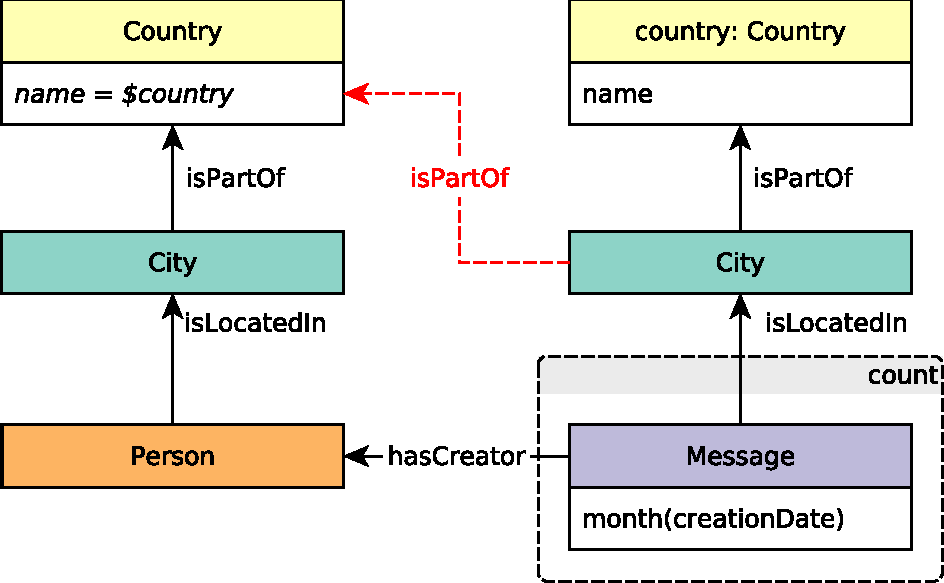
\includegraphics[scale=\patternscale,margin=0cm .2cm]{patterns/bi-read-23}
		\caption{Example graph pattern.}
		\label{fig:example-graph-pattern}
	\end{center}
\end{figure}

\paragraph{Resolving ambiguity.} Note that if the textual description and the graph pattern are different for a particular query (either due to an error or the lack of sophistication in the graphical syntax), \emph{the textual description takes precedence}.
